\section{Travail demandé}
\begin{enumerate}
  \item \q{Ecrire une fonction qui prend en argument la vitesse de rotation du bras moteur }
        \il{wm}\q{ un vecteur }\il{Tm}\q{ contenant des valeurs de $\theta_m(t)$ et qui renvoie des vecteurs }
        \il{A}\q{, }
        \il{B}\q{, }
        \il{Ap}\q{, }
        \il{Bp}\q{ et }
        \il{Cp}
        \q{ contenant $A(\theta_m)$, $B(\theta_m)$, $\dot{A}(\theta_m)$, $\dot{B}(\theta_m)$ et $\dot{C}(\theta_m)$.}

        Je commence par renommer les fonctions $cos$ et $sin$ :
        \codeFromFile{section-04/q1-1.py}

        Ensuite, comme à mon habitude, je crée un dossier \il{ressources} dans lequel je crée le fichier \il{data.py} :
        \codeFromFile{section-04/q1-2.py}

        J'importe tout ce dont j'ai besoin au début de mon fichier :
        \codeFromFile{section-04/q1-3.py}

        Puis je calcule les données demandés :
        \codeFromFile{section-04/q1-4.py}


  \item \q{En utilisant la fonction précédente, écrire une fonction qui prend en argument la vitesse de
          rotation du bras du moteur }\il{wm}\q{, l'angle de rotation maximal }\il{Tmmax}\q{ du bras du moteur, le nombre
        }\il{N}\q{ de points désirés et qui renvoie deux vecteurs, l'un, }\il{Tm}\q{ contenant les valeurs de
          $\theta_m(t)$ et l'autre, }\il{Tpv}\q{, contenant les valeurs de $\dot{\theta}_v(t)$.}

        D'abord, pour alléger la fonction demandée, je crée une fontion \il{Tpv} qui calcule $\dot{\theta}_v$ :

        \codeFromFile{section-04/q2-1.py}

        Puis je calcule les deux vecteurs demandés :

        \codeFromFile{section-04/q2-2.py}

  \item \q{Tester cette fonction pour une valeur de $\omega_m$ de $0,1 rad.s^{-1}$, et un nombre de point par
          défaut $N = 1000$. Faire afficher le graphe de $\dot{\theta}_v$ en fonction de $\theta_m$ et comparer avec les
          valeurs obtenues expérimentalement :}
        \[
          \left\{
          \begin{array}{rcl}
            \dot{\theta}_{v_{maxi}} & = & 0,088 rad.s^{-1} \\
            \theta_m                & = & 0,46 rad         \\
          \end{array}
          \right.
        \]

        Je crée la petite fonction de conversion de dergé vers radian :
        \codeFromFile{section-04/q3-1.py}

        Puis j'applique le script :
        \codeFromFile{section-04/q3-2.py}

        Et j'obtiens :

        \[
          \left\{
          \begin{array}{rcl}
            \dot{\theta}_{v_{maxi}} & \simeq & \il{0,086} \thinspace rad.s^{-1} \\
            \theta_m                & \simeq & \il{0,477} \thinspace rad        \\
          \end{array}
          \right.
        \]
        ce qui est proche des valeurs expérimentales.


        \begin{center}
          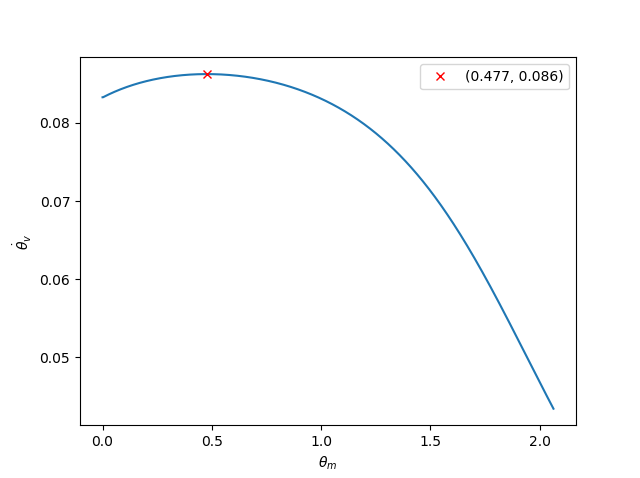
\includegraphics[scale=0.7]{section-04/q3-3.png}
        \end{center}
  \item \q{En utilisant les fonctions précédentes et en faisant évoluer $\omega_m$ sur
        l'intervalle $[0.1, 0.3]$ par pas de $0.01$, écrire le programme principal qui permet
        de trouver la valeur maximale de $\omega_m$ vérifiant le critère du cachier des charges
        (vitesse maximale autorisée par la norme pour le point le plus rapide du portail :
        $0,25 m.s^{-1}$). Rappel : $|V_{D, 3/0}| = OD. |\dot{\theta}_v|$.}

        \bigskip

        On veut la valeur $|\dot{\theta}_v|$ maximale, tout en respectant $|V_{D, 3/0}| \leq 0.25m.s^{-1}$.\\
        On rajoute la valeur maximale de $L = OD$, de $V_{D,3/0} = 0.25 m.s^{-1}$ et de $\theta_{m\_maxi} = 118.2^{\circ}$ dans le fichier \il{ressources/Data.py}
        \codeFromFile{section-04/q4-1.py}

        Fonction principale :
        \codeFromFile{section-04/q4-2.py}

        Et, en exécutant :
        \codeFromFile{section-04/q4-3.py}

        On obtient :
        \begin{result}
          $
            \left\{
            \begin{array}{rcl}
              \dot{\theta}_{v_{maxi}} & = & \il{0.14} \thinspace rad.s^{-1} \\
              V_{D, 3/0}              & = & \il{0.247} \thinspace m.s^{-1}  \\
            \end{array}
            \right.
          $
        \end{result}
\end{enumerate}
